\documentclass[11pt,reqno]{amsart}
\usepackage[margin=1in]{geometry}                % See geometry.pdf to learn the layout options. There are lots.
\geometry{letterpaper}                   % ... or a4paper or a5paper or ... 
%\geometry{landscape}                % Activate for for rotated page geometry
\usepackage[parfill]{parskip}    % Activate to begin paragraphs with an empty line rather than an indent
\usepackage{graphicx}
\usepackage{amssymb}
\usepackage{epstopdf}
\usepackage{natbib}
%\usepackage[nomarkers,nolists,figuresonly]{endfloat}
\usepackage{booktabs}

\DeclareGraphicsRule{.tif}{png}{.png}{`convert #1 `dirname #1`/`basename #1 .tif`.png}

\newcommand\independent{\protect\mathpalette{\protect\independenT}{\perp}}
\newcommand\gamij{\mathbf{\gamma_{ij}}}
\def\independenT#1#2{\mathrel{\rlap{$#1#2$}\mkern2mu{#1#2}}}
\newcommand\params{(p_M, p_{M\ell}, p_{U\ell})}
\newcommand\longparam{(L,n_1,n_2, p_M,p_{M\ell},p_{U\ell})}

\title{Bayesian Record Linkage}
\author{Rachel Anderson}
%\date{\today}                                           % Activate to display a given date or no date
\calclayout
\begin{document}
\vspace*{-1cm}
\maketitle

%Introduction

\section{Introduction}

Ask any economist who works with survey or administrative data how they handle imperfect matches when performing a one-to-one merge, and you will get a different answer.  Some pick the matches that they believe are most likely to be correct.  Some estimate the same model using multiple configurations of matched data.  Others avoid the issue entirely, by dropping all matches that are flagged during the automated merge processes in R or Stata.  There is no one-size-fits-all solution for data merging, nor a formal theory about how subjective decisions in the merging process may introduce bias or uncertainty into estimation and inference in economic models. 

This ```merging" problem of joining records from multiple data sources that describe the same entity appears in many fields, such as statistics, computer science, operations research, and epidemiology, under many names, such as record linkage, data linkage, entity resolution, instance identification, de-duplication, merge/purge processing, and entity reconciliation.    In econometrics, these topics fall under the umbrella of ``data combination", and its importance is growing with the increasing availability of large administrative datasets \citep{ridder_moffitt_2007}.  While there are many record linkage techniques, there is little understanding of how these techniques may bias inference, or how researchers should handle these issues in practice.  Examining Bayesian record linkage tools is a promising place to start, as they provide a coherent framework for incorporating uncertainty at every point of the analysis.  

In this paper, I review and implement two Bayesian record linkage procedures from \cite{larsen_rubin_2001} and \cite{sadinle_2017} to obtain a posterior distribution over the bipartite matching/sets of matches vs. non-matches. I use simulated data (and maybe a real data set if I have time).  I analyze adjustments for what makes a better match and compare them to traditional techniques.

Then, with these posteriors, I perform a basic regression analysis using methods from \cite{lahiri_larsen_2005} and \cite{tancredi_liseo_2015} \cite{tancredi_liseo_2011} about how to propagate uncertainty from the matches into a basic regression analysis.   
%also tancredi liseo 2015

I (1) review the two methods
(2) implement both, and compare results
(3) write a research plan -- how I will continue the analysis

\section{Setup}

Consider two datafiles $X_1$ and $X_2$ that record information from two overlapping sets of individuals or entities.  The files originate from two record-generating processes that may induce errors and missing values, so that identifying which individuals are represented in both $X_1$ and $X_2$ is nontrivial.  I assume that individuals appear at most once in each datafile, so that the goal of record linkage is to identify which records in files $X_1$ and $X_2$ refer to the same entities.

Suppose that files $X_1$ and $X_2$ contain $n_1$ and $n_2$ records, respectively, and without loss of generality that $n_1 \geq n_2$.  Denote also the number of entities represented in both files as $n_{M}$, so that $n_2\geq n_M \geq 0$. 

Following the probabilistic record linkage framework of \cite{fs1969}, we say that the set of ordered record pairs $X_1 \times X_2$ is the union of two disjoint sets, \textit{matches} $(M)$ and \textit{non-matches} $(U)$:
\begin{align*} M &= \{(i,j): i\in X_1, j\in X_2, i=j\} \\ U &= \{(i,j): i\in X_1, j\in X_2, i\neq j\}\end{align*} 

Hence, the formal goal of record linkage is to identify whether an arbitrary record pair $(i,j)\in X_1\times X_2$ belongs to $M$ or $U$. 

To perform this task, each record pair is evaluated according to $L$ different comparison criteria, which are the result of comparing data fields for records $i$ and $j$.  For example, if a record pair $(i,j)$ represents two individuals, the pair may be evaluated according to whether they share a first name or have the same birthday.  These comparisons are represented by a \textit{comparison vector}, $$\mathbf{\gamma_{ij}}= (\gamma_{ij}^1, \dots, \gamma_{ij}^{\ell}, \dots, \gamma_{ij}^L)$$  where each comparison field $\gamma_{ij}^{\ell}$ may be binary-valued, as in ``$i$ and $j$ have the same birthday," or use levels to account for partial agreement between strings (see \citealp{winkler90}, for details).  The models presented herein use only binary comparison vectors, however they may be extended to allow for partial agreement using the methods from \cite{sadinle_2017}.

The probability of observing a particular configuration of $\gamij$ can be modeled as arising from the mixture distribution:
\begin{equation}
P(\gamij) = P(\gamij | M) p_M + P(\gamij | U) p_U 
\label{mm}
\end{equation}
where $P(\gamma_{ij} | M)$ and $P(\gamma_{ij} | U)$ are the probabilities of observing the pattern $\gamma_{ij}$ conditional on the record pair $(i,j)$ belonging to $M$ or $U$, respectively.  The proportions $p_M$ and $p_U = 1-p_M$ are the marginal probabilities of observing a matched or unmatched pair.  Applying Bayes' Rule, we obtain the probability of $(i,j) \in M$ conditional on observing $\gamij$,
\begin{equation} P(M | \gamij) = \frac{p_M P(\gamij | M)}{P(\gamij)} \label{bayes} \end{equation}
so that if we can estimate the variables in (\ref{mm}), we can estimate the probability that any two records refer to the same entity in (\ref{bayes}).  

%good until here
As shown by \cite{fs1969}, it is possible to use the estimated probabilities to construct an ``optimal" matching, given any threshold for false positive and false negative match rates.  Conversely, the probabilities also allow us to estimate the false positive rate for any configuration of matches \citep{bda3}.  Given the usefulness of the quantities in (\ref{bayes}), the next sections will introduce two methods for estimating them.

\section{Simplifying assumptions}

Let $\mathbf{\Gamma} \equiv \{\mathbf{\gamma_{ij}}: \  (i,j) \in X_1\times X_2\}$ denote the set of comparison vectors for all records pairs $(i,j) \in X_1\times X_2$.  

\subsection{Blocking} 

Note that $\mathbf{\Gamma}$ contains potentially $n_1 \times n_2$ elements, so that calculating $\mathbf{\Gamma}$ may be computationally expensive when $X_1$ or $X_2$ is large.  In practice, researchers partition $X_1\times X_2$ into ``blocks," such that only records belonging to the same block are attempted to be linked, and records belonging to different blocks are assumed to be nonmatches.  For example, postal codes and household membership are often used to define blocks when linking census files \citep{herzog2007}.  Importantly, the blocking variables should be recorded without error, and sometimes there are none available. 

% this will need fixing:
This paper assumes that no blocking is used; or, alternatively, that records are already divided into blocks that can be analyzed independently using the methods outlined below.  

\subsection{Conditional independence} In principle, we can model,
\begin{align*} \gamij\  |\  M &\sim \text{Dirichlet}(\mathbf{\delta_M})\\
\gamij\  |\  U &\sim \text{Dirichlet}(\mathbf{\delta_U}) \end{align*}
However, there are $2^{L}-1$ possible configurations of each $\gamij$, so that $\mathbf{\delta_M}$ and $\mathbf{\delta_U}$ may be very high-dimensional if we want to allow weights to vary across different comparison criteria.

A common assumption in the literature is that the comparison fields $\ell$ are defined so that $\gamma_{ij}^{\ell}$ are independent across $\ell$ conditional on match status.  This implies:
 \begin{equation} 
 P(\gamma_{ij} | C) = \prod_{\ell=1}^L P(\gamma_{ij}^{\ell} | C)^{\gamma_{ij}^{\ell}}(1-Pr(\gamma_{ij}^{\ell} | C))^{1-\gamma_{ij}^{\ell}} \hspace{20pt} C\in \{M, U\} 
 \label{eq:condInd}
 \end{equation}
Hence the number of parameters used to describe each mixture class is reduced to $L$.  

\cite{larsen_rubin_2001} have shown how to relax this assumption using log-linear models, but for now I assume conditional independence to ease computation. 
 
 
 \section{Two Bayesian Approaches to Record Linkage}

\subsection{Mixture Models}  Since membership to $M$ or $U$ is not actually observed, a convenient way of simultaneously estimating $p_M, p_U$ and classifying record pairs as matches or non-matches is via mixture modeling, with mixture distributions $P(\gamij | M)$ and $P(\gamij | U)$.   %This approach was suggested by Bayesian approaches to record linkage have been suggested by Larsen (1999a, 2002, 2004, 2005), Fortini et al. (2002, 2000), and McGlinchy (2004).

For convenience, denote $p_{M\ell} = P(\gamma_{ij}^{\ell} | M)$ and $ p_{U\ell} = P(\gamma_{ij}^{\ell} | U)$.  Assuming conditional independence across $\ell$ (and global parameters that do not vary by block, if using blocked records), a convenient prior distribution is the product of independent Beta distributions,
 \begin{gather*}
 p_M \sim \text{Beta}(\alpha_M, \beta_M) \\
 p_{M\ell} \sim \text{Beta}(\alpha_{M\ell}, \beta_{M\ell}), \ \ell = 1,\dots, L \\
  p_{U\ell} \sim \text{Beta}(\alpha_{U\ell}, \beta_{U\ell}), \ \ell = 1,\dots, L 
 \end{gather*}
 For $i=1,\dots,n_1 \in X_1$, $j = 1, \dots, n_2 \in X_2$ define the parameter of interest as,
$$I_{ij} = \begin{cases} 1, & \text{if records $i\in X_1$ and $j\in X_2$ refer to the same entity;} \\ 0, & \text{otherwise} \end{cases} $$  
If $\params$ are known, then $P(I_{ij} = 1 | \gamij \params)$ is distributed as in (\ref{bayes}).  Alternately, if the match indicators $\mathbf{I}$ were known, the posterior distributions of $\left(p_M, \mathbf{p_{M\ell}, p_{U\ell}}\right)$ would be:

% pM | I
\begin{equation}
p_M | I \sim \text{Beta}\left(\alpha_M + \sum_{(i,j)} I_{ij},\ \beta_M + \sum_{(i,j)} (1- I_{ij})\right) 
\label{eq:pM}
\end{equation}

% pML | I 
\begin{equation}
p_{M\ell} | I \sim \text{Beta}\left(\alpha_{M\ell} + \sum_{(i,j)} I_{ij}\gamma_{ij}^{\ell},\ \beta_{M\ell} + \sum_{(i,j)} I_{ij} (1-\gamma_{ij}^{\ell})\right), \hspace{10pt} \ell = 1,\dots, L
\label{eq:pML}
\end{equation}

%pUL | I 
\begin{equation}
p_{U\ell} | I \sim \text{Beta}\left(\alpha_{U\ell} + \sum_{(i,j)}(1-I_{ij})\gamma_{ij}^{\ell},\ \beta_{U\ell} + \sum_{(i,j)}(1-I_{ij})(1-\gamma_{ij}^{\ell})\right), \hspace{10pt} \ell = 1,\dots, L
\label{eq:pUL}
\end{equation}

% \[ P(\mathbf{\Gamma} | \mathbf{I}) &= \prod_{(i,j)} P(\gamij | M)^{I_{ij}} P(\gamij | U)^{1-I_{ij}} \]

Based on these ideas, \cite{larsen_rubin_2001} proposed a Bayesian version of record linkage for the mixture model approach, that uses a Gibbs Sampling scheme\footnote{See Appendix \ref{app:simple_gibbs}} for simulating the posterior distribution of $I,\params$. 

\subsection{Beta Record Linkage}  As noted by \cite{larsen_2005}, a significant limitation of the mixture model approach is that it does not explicitly enforce one-to-one matching in the likelihood.  Intuitively, if one-to-one matching is desired, then the matching status of $(i,j)$ should depend on the the matching status of $(i,j')$ for $j\neq j'$.  The Gibbs Sampler in Appendix \ref{app:simple_gibbs} certainly violates this, since the components of $\mathbf{I}$ are sampled independently in every iteration.
 
When the goal is one-to-one matching, \cite{sadinle_2017} noted that the parameter of interest $\mathbf{I}$ is better characterized as a \textit{bipartite matching}.   Furthermore, he provides conditions under which the mixture model approach, combined with an optimal assignment of record pairs obtained from a linear sum assignment problem, produces the MLE of the bipartite matching. 

Formally, the bipartite matching can be represented as $\mathbf{Z}= (Z_1, Z_2,\dots, Z_{n_2})$, where

\[ Z_j = \begin{cases} i, & \text{if records $i\in X_1$ and $j\in X_2$ refer to the same entity;} \\
				n_1+i, & \text{if record $j\in X_2$ does not have a match in $X_1$} \end{cases} \]

This notation is also convenient computationally because it reduces the size of the matching parameter from $n_1\times n_2$ to $n_2$. 

Same as in the mixture model approach, the prior probability that $j \in X_2$ has a match is
\begin{equation} I(Z_j \leq n_1)  \overset{i.i.d}{\sim} \text{Bernoulli}(p_M), \hspace{10pt} p_M \sim \text{Beta}(\alpha_{M}, \beta_{M} \label{cond1} \end{equation}
The prior on $p_M$ implies $n_{M}(Z) = \sum_{j=1}^{n_2} I(Z_j \leq n_1)$, the number of matches according to $\mathbf{Z}$ is distributed as:
\begin{equation} n_{M}(\mathbf{Z}) \sim \text{Beta-Binomial}(n_2, \alpha_{M}, \beta_{M}) \end{equation}
after marginalizing over $p_M$.

Conditioning on $\{I(Z_j \leq n_1)\}_{j=1}^{n_2}$, all possible bipartite matchings are considered to be equally likely, so \begin{equation} Pr\left(\mathbf{Z} | n_{M}\right) = \left(\frac{n_1!}{(n_1-n_{M})!}\right)^{-1} \label{cond3} \end{equation}

Together conditions (\ref{cond1})-(\ref{cond3}) imply the following prior over $\mathbf{Z}$:
\begin{equation}Pr(\mathbf{Z} | \alpha_M, \beta_M) = \frac{(n_1-n_{M}(\mathbf{Z}))!}{n_1!}\frac{\text{Beta}(n_{M}(\mathbf{Z}) + \alpha_M,\ n_2-n_{M}(\mathbf{Z}) + \beta_M)}{\text{Beta}(\alpha_M, \beta_M)} \label{brl} \end{equation}

It is because of the prior in (\ref{brl}) that \cite{sadinle_2017} refers to his methods as \textit{beta record linkage}. 

To estimate the model, I use the Gibbs Sampling scheme outlined in \cite{larsen_2005}, which I have reproduced in Appendix \ref{app:gibbsB}.  It is very similar to the Gibbs Sampler for estimating the mixture model, however the drawing  from the conditional distribution of $\mathbf{Z}$ is significantly more challenging (and computationally intensive) than sampling from the conditional distribution of $\mathbf{I}$.  

\section{Simulation Study}

To compare the performance of the mixture model approach with the beta record linkage model, I wrote Python scripts that implement the Gibbs Samplers described in Appendices \ref{app:simple_gibbs} and \ref{app:gibbsB}.  I also wrote scripts to generate fake data using different parameter combinations so I could study how the methods perform across multiple datasets.   Detailed documentation for all relevant programs is available in \texttt{README.md} submitted with this paper. 

\subsection{Data}

For each combination of parameters in Table \ref{params}, I generated a dataset by randomly selecting $n_M = p_M^* n_2$ records from $X_2$ and $n_M$ records from $X_1$ and assigning them as matches.  

I must emphasize that this means $p_M^*$ controls the amount of overlap between the two files.  When $p_M^* = 0.9$ and $n_1=n_2 = 10$, this means all but one record in $X_2$ has a match in $X_1$.  However, these same parameter values would imply $p_M = 0.09$ according to (\ref{mm}), since there are only 9 record pairs referring to matches out of 100 possible candidate pairs.\footnote{Admittedly, this is a significant mistake on my part that I realized only after analyzing the results.}

For these record pairs, I generated $\gamij$ according to
 $$\gamma_{ij}^{\ell} \ | \ M \overset{i.i.d.}{\sim}\text{Bernoulli}(p_{M\ell}), \hspace{10pt}\ell = 1,\dots L$$ 
For the remaining $(n_1n_2 - n_M)$ record pairs, I generated $\gamij$ from
  $$\gamma_{ij}^{\ell} \ | \ U \overset{i.i.d.}{\sim}\text{Bernoulli}(p_{U\ell}), \hspace{10pt}\ell = 1,\dots L$$ 
For this paper, I tested $p_{M\ell} = 0.9$ and $p_{U\ell}=0.2$ for all $\ell$ and all datasets, however my Python programs allow for more flexible choices.  

\begin{table}[h!]
\caption{Parameter combinations and time to perform 100,000 iterations (in seconds)}
\begin{center}
\begin{tabular}{ccccccc|cc}
\toprule
 $L$ &  $n_1$ &  $n_2$ &  $p_M^*$ &  $p_M$ & $p_{M\ell}$ &  $p_{U\ell}$ & MM & BRL \\
\midrule
 2 &  10 &  10 &  0.2 & 0.02 &  0.9 &  0.2 & 237 & 4174 \\
 3 &  10 &  10 &  0.2 & 0.02 & 0.9 &  0.2 & 292 & 4315 \\
 4 &  10 &  10 &  0.2 & 0.02 & 0.9 &  0.2 & 329 & 4361 \\ 
 5 &  10 &  10 &  0.2 & 0.02 & 0.9 &  0.2 & 379 & 4417 \\ 
 2 &  20 &  20 &  0.5 & 0.05 & 0.9 &  0.2 &  900 & 14967 \\ 
 3 &  20 &  20 &  0.5 & 0.05 & 0.9 &  0.2 & 1274 & 18643 \\ 
 4 &  20 &  20 &  0.5 & 0.05 & 0.9 &  0.2 & 1490 & 18618\\
 5 &  20 &  20 &  0.5 & 0.05 & 0.9 &  0.2 & 1469 & 15470 \\
 2 &  10 &  10 &  0.9 & 0.09 & 0.9 &  0.2 &  242 & 4246 \\
 3 &  10 &  10 &  0.9 & 0.09 & 0.9 &  0.2 & 289 & 4255 \\
 4 &  10 &  10 &  0.9 & 0.09 & 0.9 &  0.2 & 334 & 4327 \\
 5 &  10 &  10 &  0.9 & 0.09 & 0.9 &  0.2 & 382 & 4249 \\
\bottomrule
\end{tabular}
\end{center}
\label{params}
\end{table}%

\subsection{Priors} This paper tests only flat priors, $(\alpha_M=\beta_M=\alpha_{M\ell}=\beta_{M\ell}=\alpha_{U\ell}=\beta_{U\ell}=1$), however, my programs allow for any valid combination of hyperparameters.  

In future tests, I would like to try restricting the following restrictions suggested by \cite{larsen_2005}:
\begin{enumerate}
\item Logically, the range of $p_M$ should be restricted to be less than or equal to the smaller of the two file sizes divided by the number of pairs under the blocking structure.  In my application, which does not use blocking, this would mean truncated any draws that violate $p_M \leq \frac{\min\{n1,n2\}}{n1n_2} = \frac{1}{n_1}$, since I assumed $n_1 \geq n_2$. 
\item The probability of a record pair agreeing on a comparison field should be no weakly greater among matches than among nonmatches.  That is, $$P(\gamma_{ij}^{\ell} | M) \geq P(\gamma_{ij}^{\ell} | U)$$ for all $\ell$.  This can be achieved by truncating the draws for $p_{U\ell}$ in the Gibbs sampler by ignoring draws that violate this condition, or by scaling $p_{M\ell}$ to be in the range $(0, p_{M\ell})$. 
\end{enumerate}

\subsection{Computation} Due to the long run time required to estimate the beta record linkage model, I performed my posterior simulation using the Adroit cluster hosted by Princeton Research Computing.   Included in my code directory is a Python script \texttt{job\_writer.py} that reads in a CSV file of parameter combinations and outputs a SLURM file that can be submitted to the cluster to run the simulations.  

For each dataset, I perform 100,000 iterations for each the mixture model and beta record linkage Gibbs samplers.  Prior to submitting these jobs to the cluster, I performed the analysis on my local machine and estimated the run time to be approximately linear in $n_1\times n_2 \times L \times $ \# iterations.  This does not seem to be entirely true on the cluster, since $(L=5, n_1 = n_2 = 20)$ completed faster than $(L=3,n_1=n_2=20)$. 

% FIX this
Finally, I compute all THINGS IN LOGS ** mention from BDA3 HERE

\section{Results}

\subsection{Mixture Model} 
To evaluate convergence for the mixture models, I look at the trace plots of $\params$.  A common pattern across all chains is that $p_M$ converges to values near 0 or 1 within a few initial draws, and then stays close to that value for all remaining draws, as in Figure \ref{mmConverge}.  Given the fact that the true values of $p_M$ are less than 0.09 for all datasets, this is not concerning.  The fact that $p_M$ sometimes converges to 1 is an artifact of the label degeneracy problem for mixture models; although I label my parameters with $M$ and $U$, my model cannot tell the difference.

Additionally, one of $\mathbf{p_{M\ell}}$ or $\mathbf{p_{U\ell}}$ oscillates between 0 and 1 for all draws, while the other oscillates between 0.15 and 0.35.  Because the values of $p_M$ are so low, $\mathbf{p_{M\ell}}$ is not well identified, and so its posterior is the same as the prior (Figure \ref{mmLarge}).  My Gibbs sampler, in turn, classifies almost all record pairs as non-matches, so that I effectively estimate the parameters $\mathbf{p_{U\ell}}$ using the entire sample. The resulting posteriors are approximately Normal, with $\hat{\mu} \approx 0.22,  \hat{\sigma} \approx 0.04$ across $p_{U\ell}$.
 
% MM trace plots
\begin{figure}[htbp]
\begin{center}
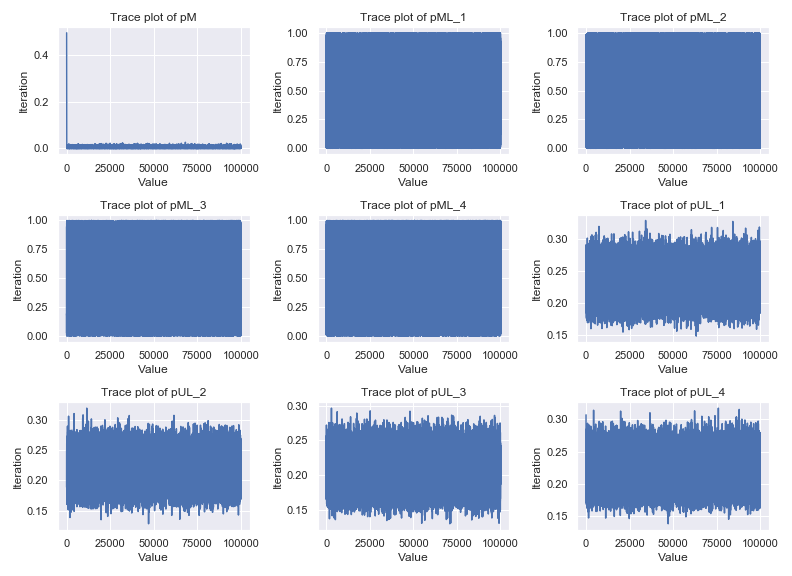
\includegraphics[width=\textwidth]{../Figures/mm/nM10/allTrace_nM10_L4.png}
\caption{Trace plots for 100,000 draws of $\params$ with true values of $\longparam = (4,20,20,0.5,0.9,0.2)$ and no burn-in}
\label{mmConverge}
\end{center}
\end{figure}

% MM  ALLparam - posterior densities
\begin{figure}[h!]
\begin{center}
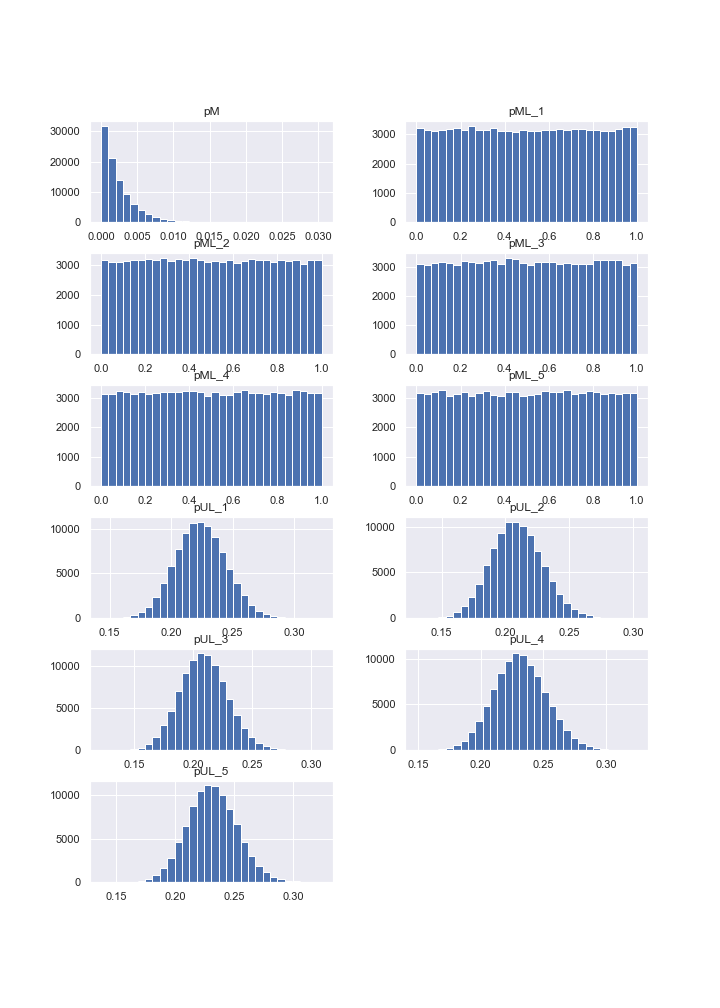
\includegraphics[width=0.9\textwidth]{../Figures/mm/nM10/allParam_nM10_L5.png}
\vspace{-40pt}
\caption{Histogram of 100,000 draws (burn-in = 5,000) from mixture model for all parameters with true parameter values $(L, n_1, n_2, p_M, p_{M\ell}, p_{U\ell}) = (5, 20, 20, 0.5, 0.9, 0.2)$ and independent, flat priors}
\label{mmLarge}
\end{center}
\end{figure}


\subsection{Beta Record Linkage}  Figure \ref{bpmTrace} shows the trace plots for $\params$ and the likelihood of $Z$ from the last 15,000 draws.  It appears that $p_{U\ell}$ mixes well, but that there are slow-moving trends in $p_M, p_{M\ell}$ and the likelihood.  This suggests that the chains have not converged. 

\cite{sadinle_2017} uses Beta Record Linkage with $n_1 = 4,430, n_2 = 1,324$ which gives $5,852,080$ record pairs.  He finds that he has converged after just 2,000 iterations of the Gibbs Sampler based on Geweke's convergence diagnostic as implemented in \texttt{R} package \texttt{coda}.  In future versions of this paper, I will explore how to apply similar functions to my output, or write a custom module that calculates the appropriate convergence criteria from \cite{brooks_gelman_1998} and  \cite{gelman_rubin_1992}.

%bpm - trace plots
\begin{figure}[htbp]
\begin{center}
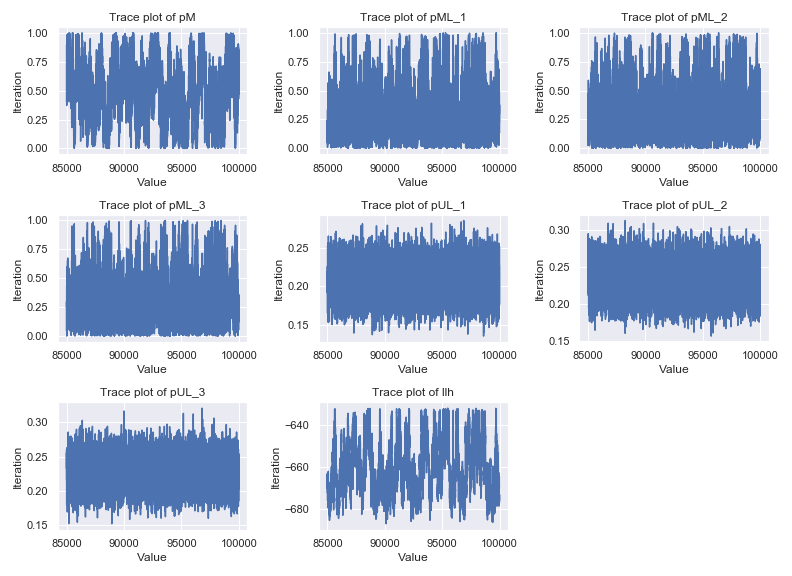
\includegraphics[width=\textwidth]{../Figures/bpm/nM10/allTrace_nM10_L3.png}
\caption{Trace plot of draws 85,000-100,000 for $\params$ and the likelihood of $Z$ from a Beta Record Linkage model with true parameters $(L, n_1, n_2, p_M, p_{M\ell}, p_{U\ell}) = (5, 20, 20, 0.5, 0.9, 0.2)$ }
\label{bpmTrace}
\end{center}
\end{figure}

\subsubsection{Matching and matching weights, Posteriors}

% NEED TO LOOK AT THE IMPLIED WEIGHTS FROM THIS MODEL

% figures for nM = 10, dim(Gamma) = 200 pM =0.5, L = 5
% mm 

\subsection{Posterior Densities}
The posterior densities for $p_{U\ell}$ in Figures \ref{mmLarge} and \ref{bpmLarge} are virtually identical for both models.  This is true for all combinations of parameters (although, as mentioned above, sometimes the $U$ and $M$ is flipped in the mixture model for $L$ small).  In the Beta Record Linkage model, the posterior density of $p_M$ remains rather flat, and the posterior densities for $p_{M\ell}$  look like a $\chi^2$ distribution. 


%bpm - posterior densities
\begin{figure}[h!]
\begin{center}
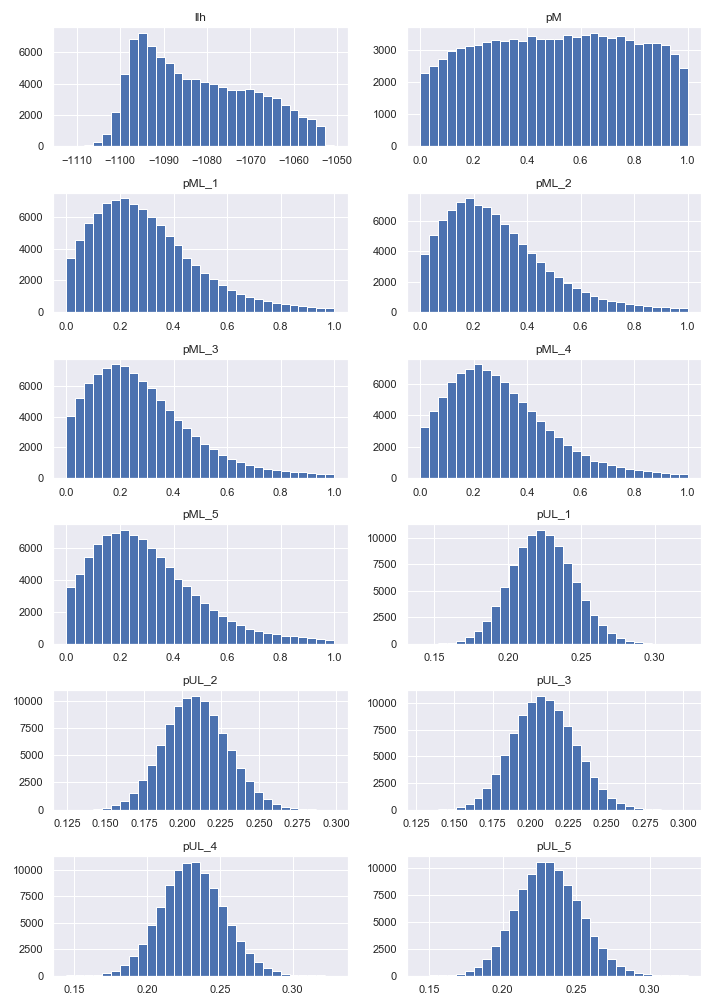
\includegraphics[width=0.9\textwidth]{../Figures/bpm/nM10/allParam_nM10_L5.png}
\caption{Histogram of 100,000 draws (burn-in = 5,000) from Beta Record Linkage model for all parameters and likelihood of $Z$ with true parameter values $(L, n_1, n_2, p_M, p_{M\ell}, p_{U\ell}) = (5, 20, 20, 0.5, 0.9, 0.2)$ and independent, flat priors}
\label{bpmLarge}
\end{center}
\end{figure}

\subsection{Beta Record Linkage}
% z - barplot

\begin{figure}[h!]
\begin{center}
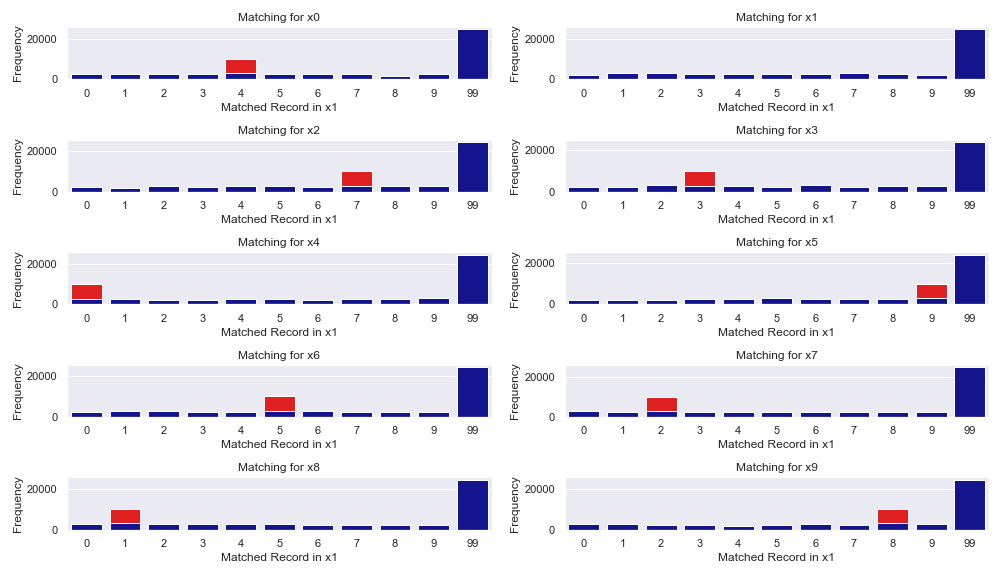
\includegraphics[width=\textwidth]{../Figures/bpm/nM9/ZmatchesnM9_L3.png}
\caption{Histogram of $Z$ draws for bipartite matching from a Beta Record Linkage model with true parameters $(L, n_1, n_2, p_M, p_{M\ell}, p_{U\ell}) = (3, 10, 10, 0.9, 0.9, 0.2)$ }
\label{Ztrace}
\end{center}
\end{figure}

\subsubsection{Posterior match probabilities} 

The estimated posterior probability of $(i,j) \in M$ is:
$$ \frac{\# \text{ iterations that } Z_j = i}{\text{total \# of iterations}} $$
for all $(i,j)\in X_1\times X_2$.  Figure \ref{Ztrace} shows that even when almost all records have a match $(p_M = 0.9)$, the posterior probability that any record is assigned a match is low.  Conditional on being assigned a match in a draw, however, the posterior seems to slightly favor the correct match (Figure \ref{ZtraceCond}) so that if we used a decision rule to assign matches, some of the matches may be correctly assigned.  Given that the chain has not converged, this seems to be promising, albeit not ideal. 

\begin{figure}[h!]
\begin{center}
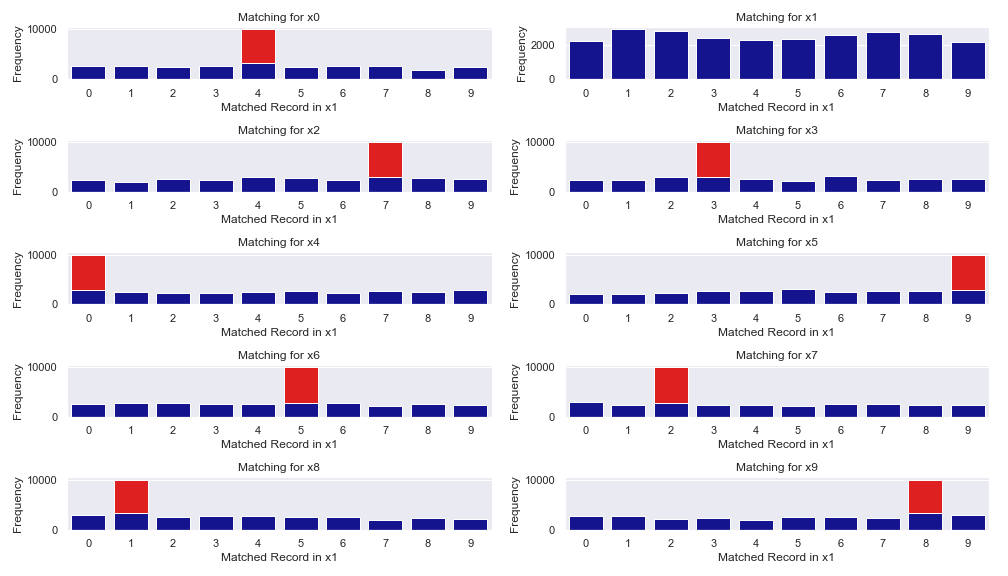
\includegraphics[width=\textwidth]{../Figures/bpm/nM9/ZmatchesnM9_L3_cond.png}
\caption{Histogram of $Z$ draws for bipartite matching (conditional on being matched) from a Beta Record Linkage model with true parameters $(L, n_1, n_2, p_M, p_{M\ell}, p_{U\ell}) = (3, 10, 10, 0.9, 0.9, 0.2)$ }
\label{ZtraceCond}
\end{center}
\end{figure}


\section{Discussion}

%%% WHERE TO PUT
\subsection{Interpreting the results}  For a candidate pair $(i,j)$, the posterior probability of a match is $P(I_{ij}  = 1 | p_M, p_{M\ell}, p_{U\ell}) = \frac{1}{K}\sum_k I_{ij}^{(k)}$.  Options for designating matches are to (1) designate all candidate pairs exceeding a cutoff as matches, or (2) use a linear program to enforce one-to-one matching. 


\subsection{Limitations}
\begin{enumerate}
\item There is no guarantee that the clusters will correspond to matches and non-matches.  This is a more general criticism about using mixture models, which suffer from this identification problem.  In practice, 3-component mixtures tend to work better, even though theoretically we would like two.  Winkler (2002) mentioned conditions for the mixture model to give good results: the proportion of matches should be greater than 5\%, the classes of matches and non-matches should be well-separated, typographical errors must be relatively low, there must be redundant fields that overcome errors in other fields, among others. 
\item Many-to-one matches can still happen unless the linear sum assignment is used.  Even if mixture model is fitted with the one-to-one constraint, the FS decision rule alone may lead to many-to-many assignments.  The linkage decision for the pair $(i,j)$ not only depends on $\gamma_{ij}$ but on the other pairs. 
\end{enumerate}


 Larsen (2012) notes that it is also possible to specify a prior distribution over the whole probability vector associated with the set of comparison vectors $\gamma$ as two Dirichlet distributions:
 \begin{gather*}
  Pr(\gamma | M) \sim \text{Dirichlet}(\delta_M) \\
 Pr(\gamma | U) \sim \text{Dirichlet}(\delta_U)
 \end{gather*}

\subsection{Enforcing one-to-one assignment}

The FS decision rule does not enforce the maximum one-to-one assignment that is desirable in many economic applications.  In practice, the optimal assignment of record pairs is obtained by solving the linear sum assignment problem: 
\begin{gather*}
%fix the fact that DELTA w_{ij} here is different than above
\max_{\Delta} \sum_{i=1}^{n_1}\sum_{j=1}^{n_2} w_{ij} \Delta_{ij}\\
\text{subject to } \Delta_{ij} \in \{0,1\}; \sum_{i=1}^{n_1} \Delta_{ij} \leq 1, \ j=1, \dots, n_2 \\ \text{and } \sum_{j=1}^{n_2} \Delta_{ij} \leq 1, \ i=1, \dots, n_1 
\end{gather*} 

where the constraints ensure that $\Delta$ represents a bipartite matching.  The output of this step is a bipartite matching that maximizes the sum of the weights $w_{ij}$ among matched pairs, and the pairs that are not matched.  Sadinle (2017) shows that this can be thought of as the MLE under the assumption that the comparison vectors are conditionally independent given the bipartite matching. %try to understand this  
%% NOT SURE WHERE TO PUT


\subsection{How to improve the results by making more prior restrictions}

It is expected that the probability of agreeing on an individual field of comparison is higher for matches than for nonmatches:
$$Pr\left(\gamma_{ij}^{\ell} = 1 |\ (i,j)\in M\right) \geq Pr\left(\gamma_{ij}^{\ell} = 1 |\ (i,j) \in U\right) $$ 
\subsection{Results} Some plots will go here. 



This method does not perform well, even when I impose strong priors and set initial parameter values equal to the truth.   First, the posterior for $p_M$ is heavily skewed toward 1 when I sample $I$ using the formula in Step 1.  This corresponds with high posterior probabilities of $I(a,b)$, which may imply large false positive matching rates if threshold is set too low. 

This issue reflects the fact that updates to $(p_M, p_{M\ell}, p_{U\ell})$ depend on assignments of $I(a,b)$. The $sample_I$ function is too quick to assign matches.  This may result from the fact that I use two clusters, and that once $p_{U\ell}$ probabilities get set low, the chain cannot recover.  I test this issue by adding 1 to the denominator of the Bernoulli parameter in Step 1:

$$p \equiv Pr(\ I(a,b)^{(k+1)}=1\ |\ \gamma(a,b)) = Pr(\ M\  |\  \gamma(a,b)) = \frac{p_M^{(k)}Pr(\ \gamma(a,b)\ |\ M)}{Pr(\gamma(a,b)) + 1} $$ 

This change prevents $p_M$ from converging to 1 <span style="color:blue">(but I need to write more tests) </span>

My results are extremely sensitive to a choice of prior! Choosing the prior will be important to explore. 

Could I sample from the joint distribution of $(p_M, p_{M\ell}, p_{U\ell})\ | I$?  Could I model as Dirichlet?

Ultimately it is not worth the time and energy trying to fix this broken method so now I focus on the bipartite matching, which will fix many of these issues.


% Some literature
\section{Dicussion/Literature}

Other option is to use training data to obtain the weights.  Another is to apply mixture models to the comparison vectors directly.  This latter method is favorable because in many contexts training data is not available, or creating a sufficiently large, representative training data set is costly.  

Referee for Belin (93): ``every gain which is achieved by a superior record linkage procedure must be justified by the cost of implementing that procedure". 


The record linkage literature can be divided into two categories, broadly.  The first are those who develop methods to perform matches that are in some way ``optimal" -- defined by reducing false match rates, or in terms of speed.  The second, where this work will eventually fall, is studying how to incorporate uncertainty from the matching process into the subsequent analysis.  Rarely are we interested in the match itself, but the analysis produced using matched data.  
\subsection{Methods people}
Larsen (2005) shows how to use a hierarchical Bayesian model to allow for matching probability of agreeing on fields of information to vary by block (but share a hyperprior $(\log(\alpha_s/\alpha_s+\beta_s) \sim \mathcal{N})$.  He also shows one-to-one restrictions.  Now $n_{12}$, the number of matches is:
\[ n_{m} \sim Binomial(n_2, p_m) \] 
where $p_m \sim Beta(\alpha_m, \beta_m)$ as before. The prior distribution for the set of matches, is uniform over the space of possible matching configurations. Suggests doing linear sum assignment procedure at each step.  %Read Appendix B

\subsection{Experimental}
Belin (1993): Performance of record-linkage procedure can depend on a number of factors, including:
\begin{enumerate}
\item Choice of matching variables
\item Choice of blocking variables
\item Assignment of weights to agreement or disagreement on various matching variables
\item Handling of close but not exact agreement between matching variables
\item Handling of missing data in one or both of a pair of records
\item Algorithm for assigning candidate matches
\item Choice of cutoff weight above which record pairs will be declared matched
\item The site or setting from which data are obtained
\end{enumerate}
In the Bayesian, case we don't need to declare anyone matched, could calculate the probability of  ``model" (match) space explored via Geweke and then use this to calculate proper weights on reviewed matches?  
\subsection{bias people}
Scheuren and Winkler (1993) and Lahiri and Larsen (2005) propose bias-corrected estimators of coefficients in a linear regression model given data from a probabilistically linked file. 

Chipperfield et al. (2011) consider the analysis of linked binary variables.

Building on Chambers (2009), Kim and Chambers (2012a, 2012b) (referred to as KC hereafter) investigate the analysis of linked data using a more general set of models fitted using estimating equations.

Kim and Chambers (2012b) review recent development in inference for regression parameters
using linked data.

Chipperfield and Chambers (2015) describes a bootstrap approach to inference using estimating equations that is based on probabilistically linked data where the linked data file is created under the 1-1 constraint.  They say this of the previous papers: 

\begin{quote}
Linkage models form the key feature of all of the above approaches. The linkage model
describes the probability that a record on one file is linked to each of the records on another
file. For a linkage model to be useful, it must properly take into account how records were
linked. SW and LL do not allow for 1-1 linkage, where every record on one file is linked to
a distinct and different record on the other, or for linkage in multiple passes or stages,
both of which are commonly used in probabilistic record linkage. In theory, KC allows
for 1-1 linkage, but imposes strong constraints on the linkage model in order to do so.
KC also requires a clerical sample to estimate the parameters of the linkage model,
something which is not always available in practice and which itself can be subject to
measurement errors.
\end{quote}

In a Bayesian approach none of this necessary maybe. 

\section{Bipartite matching}
Bayesian approaches of \cite{fortini2001} and Larsen (2002, 2005, 2010) improve the mixture model implementation by properly treating the parameter of interest as a bipartite matching, which relaxes the assumption that record pairs' matching status is independent of one another.  The setup is as follows:

Two sets: $X = \{x_1, \dots, x_{n1}\}$ and $Y = \{y_1, \dots, y_{n2}\}$. The goal is to find an assignment of items so that every item in $X$ is matched to exactly one item in $Y$ and no two items share the same match.  An assignment corresponds to a permutation $\pi$ where $\pi$ is a one-to-one mapping (check?) $\{1, \dots, n_1\} \to \{1, \dots, n_2\}$ mapping each item in $X$ to its match in $Y$.  We define $\pi(i) = j$ to denote the index of a match $y_{\pi(i)} = y_j$ for an item $x_i$, and $\pi^{-1}(j) = i$ to denote the reverse (if it exists). 

Uncertainty over assignments expressed as:
\[ P(\pi | \theta)  = \frac{1}{Z(\theta)} \exp(-E(\pi,\theta))\]
%\subsection{}


\section{Priors} 
It is expected that the probability of agreeing on an individual field of comparison is higher for matches than for non-matches is $P(\gamma_k(a,b) = 1 | (a,b) \in M) > P (\gamma_k(a, b) = 1 | (a,b) \in U) $.  And the probability of a match $p_M$ is less than or equal to the minimum file size divided by the number of possible pairs.  


%Data discription
\section{Datasets}
The techniques are tested first using a synthetic data generator developed by Christen and Pudjijono (2009) and Christen and Vatsalan (2013), and then with two real datasets from Enamorado (2018) and Enamorado, Fifield and Imai (2018). 
\begin{enumerate}
\item In the first empirical application I merge two datasets on local-level candidates for the 2012 and 2016 municipal elections in Brazil.  Each dataset contains more than 450,000 observations with a perfectly-recorded unique identifier, the Brazilian individual taxpayer registration identification number (called the \textit{Cadastro de Pessoas F\'isicas}).  All other common identifiers are manually entered into the database, so they may contain errors.  

\item In the second application, I merge the 2016 American National Election Study(ANES) with a nationwide voter file containing over 160 million voter records.  
\end{enumerate}
%(CHECK THIS ETC) To be written. 



\newpage
% Appendix -- notes on computation 

\bibliography{linkage_bib}
\bibliographystyle{chicago}

% appendix begins here
\newpage
\appendix
\section{Appendix}

\subsection{Gibbs Sampler \citep{larsen_2005}}
\label{app:simple_gibbs}
\begin{enumerate}
\item Specify parameters for the prior distributions.  Choose initial values of $\left(p_M^{(0)}, p_{M\ell}^{(0)}, p_{U\ell}^{(0)}\right)$ for $\ell=1,\dots L$.  

\item Repeat the following steps numerous times until the distribution of draws has converged to the posterior distribution of interest:
\begin{enumerate}

\item Using the current values of $\left(p_M^{(k)}, p_{M\ell}^{(k)}, p_{U\ell}^{(k)}\right)$, draw $I_{ij}^{(k+1)}$ for each $(i,j)$ candidate pair as an independent draw from a Bernoulli distribution with parameter
\begin{equation}
Pr\left( I_{ij}^{(k+1)}=1 \Big| \gamma_{ij}\right) = Pr\left(M | \gamma_{ij}\right) = \frac{p_M^{(k)}Pr\left(\gamma_{ij} | M, p_{M\ell}^{(k)} \right)}{Pr\left(\gamma_{ij} \Big | p_M^{(k)}, p_{M\ell}^{(k)}, p_{U\ell}^{(k)}\right)}
\end{equation} where 

$$ Pr\left(\gamma_{ij} | M, p_{M\ell}^{(k)} \right) = \prod_{\ell=1}^L  \left(p_{M\ell}^{(k)}\right)^{\gamma_{ij}^{\ell}}\left(1-p_{M\ell}^{(k)}\right)^{1-\gamma_{ij}^{\ell}}$$ and the denominator is calculated according to (\ref{mm}) above. 
\item Draw a value of $p_M^{(k+1)}$ from (\ref{eq:pM}).
\item Draw values of $\{p_{M\ell}^{(k+1)}\}_{\ell=1}^L$ independently from (\ref{eq:pML}). 
\item Draw values of $\{p_{U\ell}^{(k+1)}\}_{\ell=1}^L$ independently from (\ref{eq:pUL}). 
\end{enumerate}
\item Stop once the algorithm has converged.  Criteria for Convergence ARE X Y Z. %Convergence of the algorithm can be monitored by comparing distributions from multiple independent series as suggested by Gelman and Rubin (1992) and Brooks and Gelman (1998).
\end{enumerate}

\subsection{Gibbs sampler for bipartite matching \citep{larsen_2005}}
\label{app:gibbsB}
\begin{enumerate} 
\item Pick an initial values of $p_M, p_{M\ell}, p_{U\ell}$ and a valid configuration of $Z$.  Repeat the following until convergence:
\begin{enumerate} 
\item Draw $p_M$ from $$ p_M\ |\ Z \sim \text{Beta}(\alpha_M + n_{M}(Z),\ \beta_M + n_{2} - n_{M}(Z)) $$ Note this is same as before. 

\item  Draw $p_{M\ell}$ and $p_{U\ell}$ from their conditional distributions (same as before).

\item Use Metropolis-Hastings algorithm to draw values of $Z$ and $n_{M}(Z)$ from their full conditional distributions. 

\end{enumerate}

\item Stop when converged. 
\end{enumerate}



I implement the incremental method for modifying $n_M$ and $Z$ via the Metropolis-Hastings steps outlined in the appendix of Larsen (2005).  As Larsen notes, there are various Gibbs and Metropolis-Hastings sampling procedures that could generate draws from the target distribution, however most are computationally infeasible.  The following procedure is designed to cover the space of possible configurations and to produce higher probabilities of change across iterations.  

The full conditional distribution of $(n_m, Z)$ is:
\begin{equation} 
Pr\left(n_m, Z | \gamma, p_{M\ell}, p_{U\ell}, p_M, \alpha, \beta \right) \propto Pr(n_m | p_M) Pr(Z | n_M) Pr\left(\gamma | Z,  \{p_M{\ell}, p_{U\ell}\}_{\ell=1}^L, p_M, \alpha, \beta \right) \label{nmZ} \end{equation}
This is used to calculate the jump probabilities $P(n_M, Z) $ in the moves below.  For all types of moves, there are more clever ways to select which pairs to add, drop, or switch, however these are computationally expensive.  Future steps may include optimizing these steps, although ACCEPTANCE PROBABILITY IS PRETTY GOOD %look this up

\textbf{Move 1: $n_M^* = n_M - 1 $ }

A pair $(i,j)$ is picked at random from the set of matched record pairs according to the current configuration of $Z$ with equal probabilities.  The probability of picking pair $(i,j)$ is $(n_M)^{-1}$. 

The inverse move is to add the deleted pair of records to the set of designated matches.  If a non-matching pair is selected at random with equal probabilities, the probability of selecting the dropped match is $\left((n_1 - n_M + 1)(n_2 - n_M + 1)\right)^{-1}$.  Hence the acceptance probability for the Metropolis-Hastings algorithm is:
\[ \min \left\{ 1, \frac{Pr\left(n_M^*, Z^* | \text{ current parameter values}\right)  n_M}{Pr\left(n_M, Z | \text{ current parameter values}\right) (n_1 - n_M + 1)(n_2 - n_M + 1)}\right\} \] 

\textbf{Move 2: $n_M^* = n_M + 1 $ }

A pair $(i,j)$ is selected at random from the set of non-matches according to the current configuration of $Z$ with probability $\left((n_1-n_M)(n_2-n_M)\right)^{-1}$.  

The inverse move is to delete a pair of records from the set of designated matches with equal probability $n_M^{-1}$ for each pair.  This implies the acceptance probability for the Metropolis-Hastings algorithm:

\[ \min \left\{ 1, \frac{Pr\left(n_M^*, Z^* | \text{ current parameter values}\right)(n_1 - n_M)(n_2 - n_M)}{Pr\left(n_M, Z | \text{ current parameter values}\right)(n_M + 1)} \right\} \] 

\textbf{Move 3: $n_M^* = n_M$, but $Z$ changes} 

There are three variations of this move to consider. 

\textbf{Move 3.1: Two matches switch pairings}

Two matched pairs $(i,j)$ and $(k, l)$ are selected at random from the set of matched pairs according to the current configuration of $Z$.   Then the new pairs $(i,l)$ and $(k,j)$ are assigned as matches, and the old pairs $(i,j)$ and $(k,l)$ are assigned non-match status. 

The reverse move is to undo the switch, so that the acceptance probability of the M-H algorithm is
\[ \min \left\{ 1, \frac{Pr(\gamma_{il} | M) Pr(\gamma_{kj} | M) Pr(\gamma_{ij} | U) Pr(\gamma_{kl} | U)}{Pr(\gamma_{ij} | M) Pr(\gamma_{kl} | M) Pr(\gamma_{il} | U) Pr(\gamma_{kj} | U)} \right\} \] 

\textbf{Move 3.2: A matched pair replaces one of its matching records with a non-matching record}

A matched pair $(i,j)$ is chosen with uniform probability $(n_M)^{-1}$ from the set of matches.  With probability $1/2$, $i\in X_1$ is assigned a new match at random; otherwise, $j\in X_2$ is assigned a new match at random.

The new match is selected at random from the corresponding set of unmatched records in $X_1$ or $X_2$, according to whether $i$ or $j$ is dropped.   If the record $i \in X_1$ is replaced through random selection with $k \in X_1$ then the M-H acceptance probability is
\[ \min \left\{ 1, \frac{Pr(\gamma_{kj} | M) Pr(\gamma_{ij} | U)}{Pr(\gamma_{ij}| M) Pr(\gamma_{kj} | U)} \right\} \]

If a record $j\in X_2$ is replaced through random selection with $l \in X_2$, then the M-H acceptance probability is 
\[ \min \left\{1, \frac{Pr(\gamma_{il} | M) Pr(\gamma_{ij} | U)}{Pr(\gamma_{ij} | M) Pr(\gamma_{il} | U)} \right\} \]

\textbf{Move 3.3 A matched pair is deleted and two unmatched records are paired}

A matched pair $(i,j)$ is selected at random from the set of matched records according to current configuration $Z$ with equal probability.  An unmatched pair $(k,l)$ is selected at random from the set of unmatched candidate pairs with equal probability.   The acceptance probability for the M-H algorithm is

\[ \min \left\{1,  \frac{Pr(\gamma_{kl} | M)Pr(\gamma_{ij} | U) n_M}{Pr(\gamma_{ij} | M) Pr(\gamma_{kl} | U) (n_1 - n_M)(n_2 - n_M)} \right\} \]

\subsection{Notes on computation/implementation}

Following the advice of (Gelman ref), all probabilities for the algorithm above are computed first in logs and later exponentiated to calculate the jump probability to avoid numerical overflow or underflow. 

Unless otherwise noted, simulations were conducted on Adroit computing, with this machine.  


\end{document}  